\documentclass[12pt]{article}

% -- Packages --
\usepackage{graphicx}
\graphicspath{{images/}}
\usepackage{fancyhdr}
\usepackage{vmargin}
\usepackage{subfig}
\usepackage{lipsum}
\usepackage{color}
\usepackage{url}

\usepackage[colorlinks]{hyperref}
% --

% NO TOUCHY
%------------------------------------------------------------------
\setmarginsrb{3 cm}{2.5 cm}{3 cm}{2.5 cm}{1 cm}{1.5 cm}{1 cm}{1.5 cm}
\pagestyle{fancy}
\fancyhf{}
\cfoot{\thepage}
%------------------------------------------------------------------


\begin{document}

% -- TITLE PAGE --
\begin{titlepage}
	\centering
    \vspace*{0.5 cm}
    
\includegraphics[scale = 0.5]{unibas_logo.jpeg}\\[1.0 cm]
    \textsc{\LARGE  The 2016 US elections and suicide rates in the US}\\[2.0 cm]
    \textsc{ COMPUTER SCIENCE DEPARTMENT}\\[0.2 cm]
	\textsc{DATABASES - \textbf{P3}: Analysis and visualisation}\\[0.2cm]
	\textsc{\Large FS 2019}\\[0.5 cm]
	\rule{\linewidth}{0.2 mm} \\[0.4 cm]

	\begin{minipage}{0.4\textwidth}

			\begin{flushright}
			\emph{STUDENT IDS :} \\
				Rik De Graaf {\color{red}12345678}\linebreak
			Travis Rivera Petit 15-117-427\linebreak
		\end{flushright}
	\end{minipage}\\[2 cm]


	\vfill

\end{titlepage}
% --

%\tableofcontents
%\pagebreak


\section{INTRODUCTION}
{\color{red}problem}\\
"To what extent have the result of the US 2016 presidential
elections affected the suicide rates in the United States?"

{\color{red} analysis goals}\\
The rise of social media has given people from all different
backgrounds a plattform with which to share their thoughts
and feelings online leaving them avaiable for anyone to read.
This phenomenon gives society yet another tool for analysing
people's mass behavior; after all, if many individuals share
similar posts online, it may be a sign that something
is going on.
This becomes particualrly interesting
when important events that affect everyone in a contry take
palce.

After the last US elections,
some were hearly displeased and others
satisfied, this friction has been pronounced by the fact
that the controvesial figure Donald Trump has taken over
the presiency of the United States since 2016.

Many opposers of Trump did not stop at Twitter or Reddit, they
took it up to themselves to go out and protest on the streets.

Our aim is to use information about protests, riots, and
related events together with the results of the elections
and the suicide rates to make a conty-level investigation
regarding the question above.



%{\color{red} sources}\\

%{\color{red}problem}\\
"To what extent have the result of the US 2016 presidential
elections affected the suicide rates in the United States?"

{\color{red} analysis goals}\\
The rise of social media has given people from all different
backgrounds a plattform with which to share their thoughts
and feelings online leaving them avaiable for anyone to read.
This phenomenon gives society yet another tool for analysing
people's mass behavior; after all, if many individuals share
similar posts online, it may be a sign that something
is going on.
This becomes particualrly interesting
when important events that affect everyone in a contry take
palce.

After the last US elections,
some were hearly displeased and others
satisfied, this friction has been pronounced by the fact
that the controvesial figure Donald Trump has taken over
the presiency of the United States since 2016.

Many opposers of Trump did not stop at Twitter or Reddit, they
took it up to themselves to go out and protest on the streets.

Our aim is to use information about protests, riots, and
related events together with the results of the elections
and the suicide rates to make a conty-level investigation
regarding the question above.



%{\color{red} sources}\\


\section{SOURCE MATERIAL}
everything about our data sets and how we go about modeleing it.
The ER diagrams and such belong here.

%everything about our data sets and how we go about modeleing it.
The ER diagrams and such belong here.


\section{INTEGRATION}
The GDELT data subset we use in this project consists of sixty
three thousand csv files, where each file takes somewhere between
800 KB and 1.5 MB of storage.

On our P2 hand-in we include a script
(/gdelt/download.py) that downloads each csv file
and edits the filenames for further processing.
If a file is found to be corrupt, it is not downloaded and
the index of the file is saved in a .txt file
(/gdelt/bad\_indices.txt).

The dataset consists of sixty attributes and the domain of
each attribute is in detail on the official handbook
{\color{red}{citation}}.

Moving on, the suicide rate dataset can be obtained from
the Centers for Disease Control and Prevention
website \cite{suicide_website}.

The election results dataset is straightforward, it can be
obtained on {\color{red}{todo}}.

\begin{figure}
	\centering
	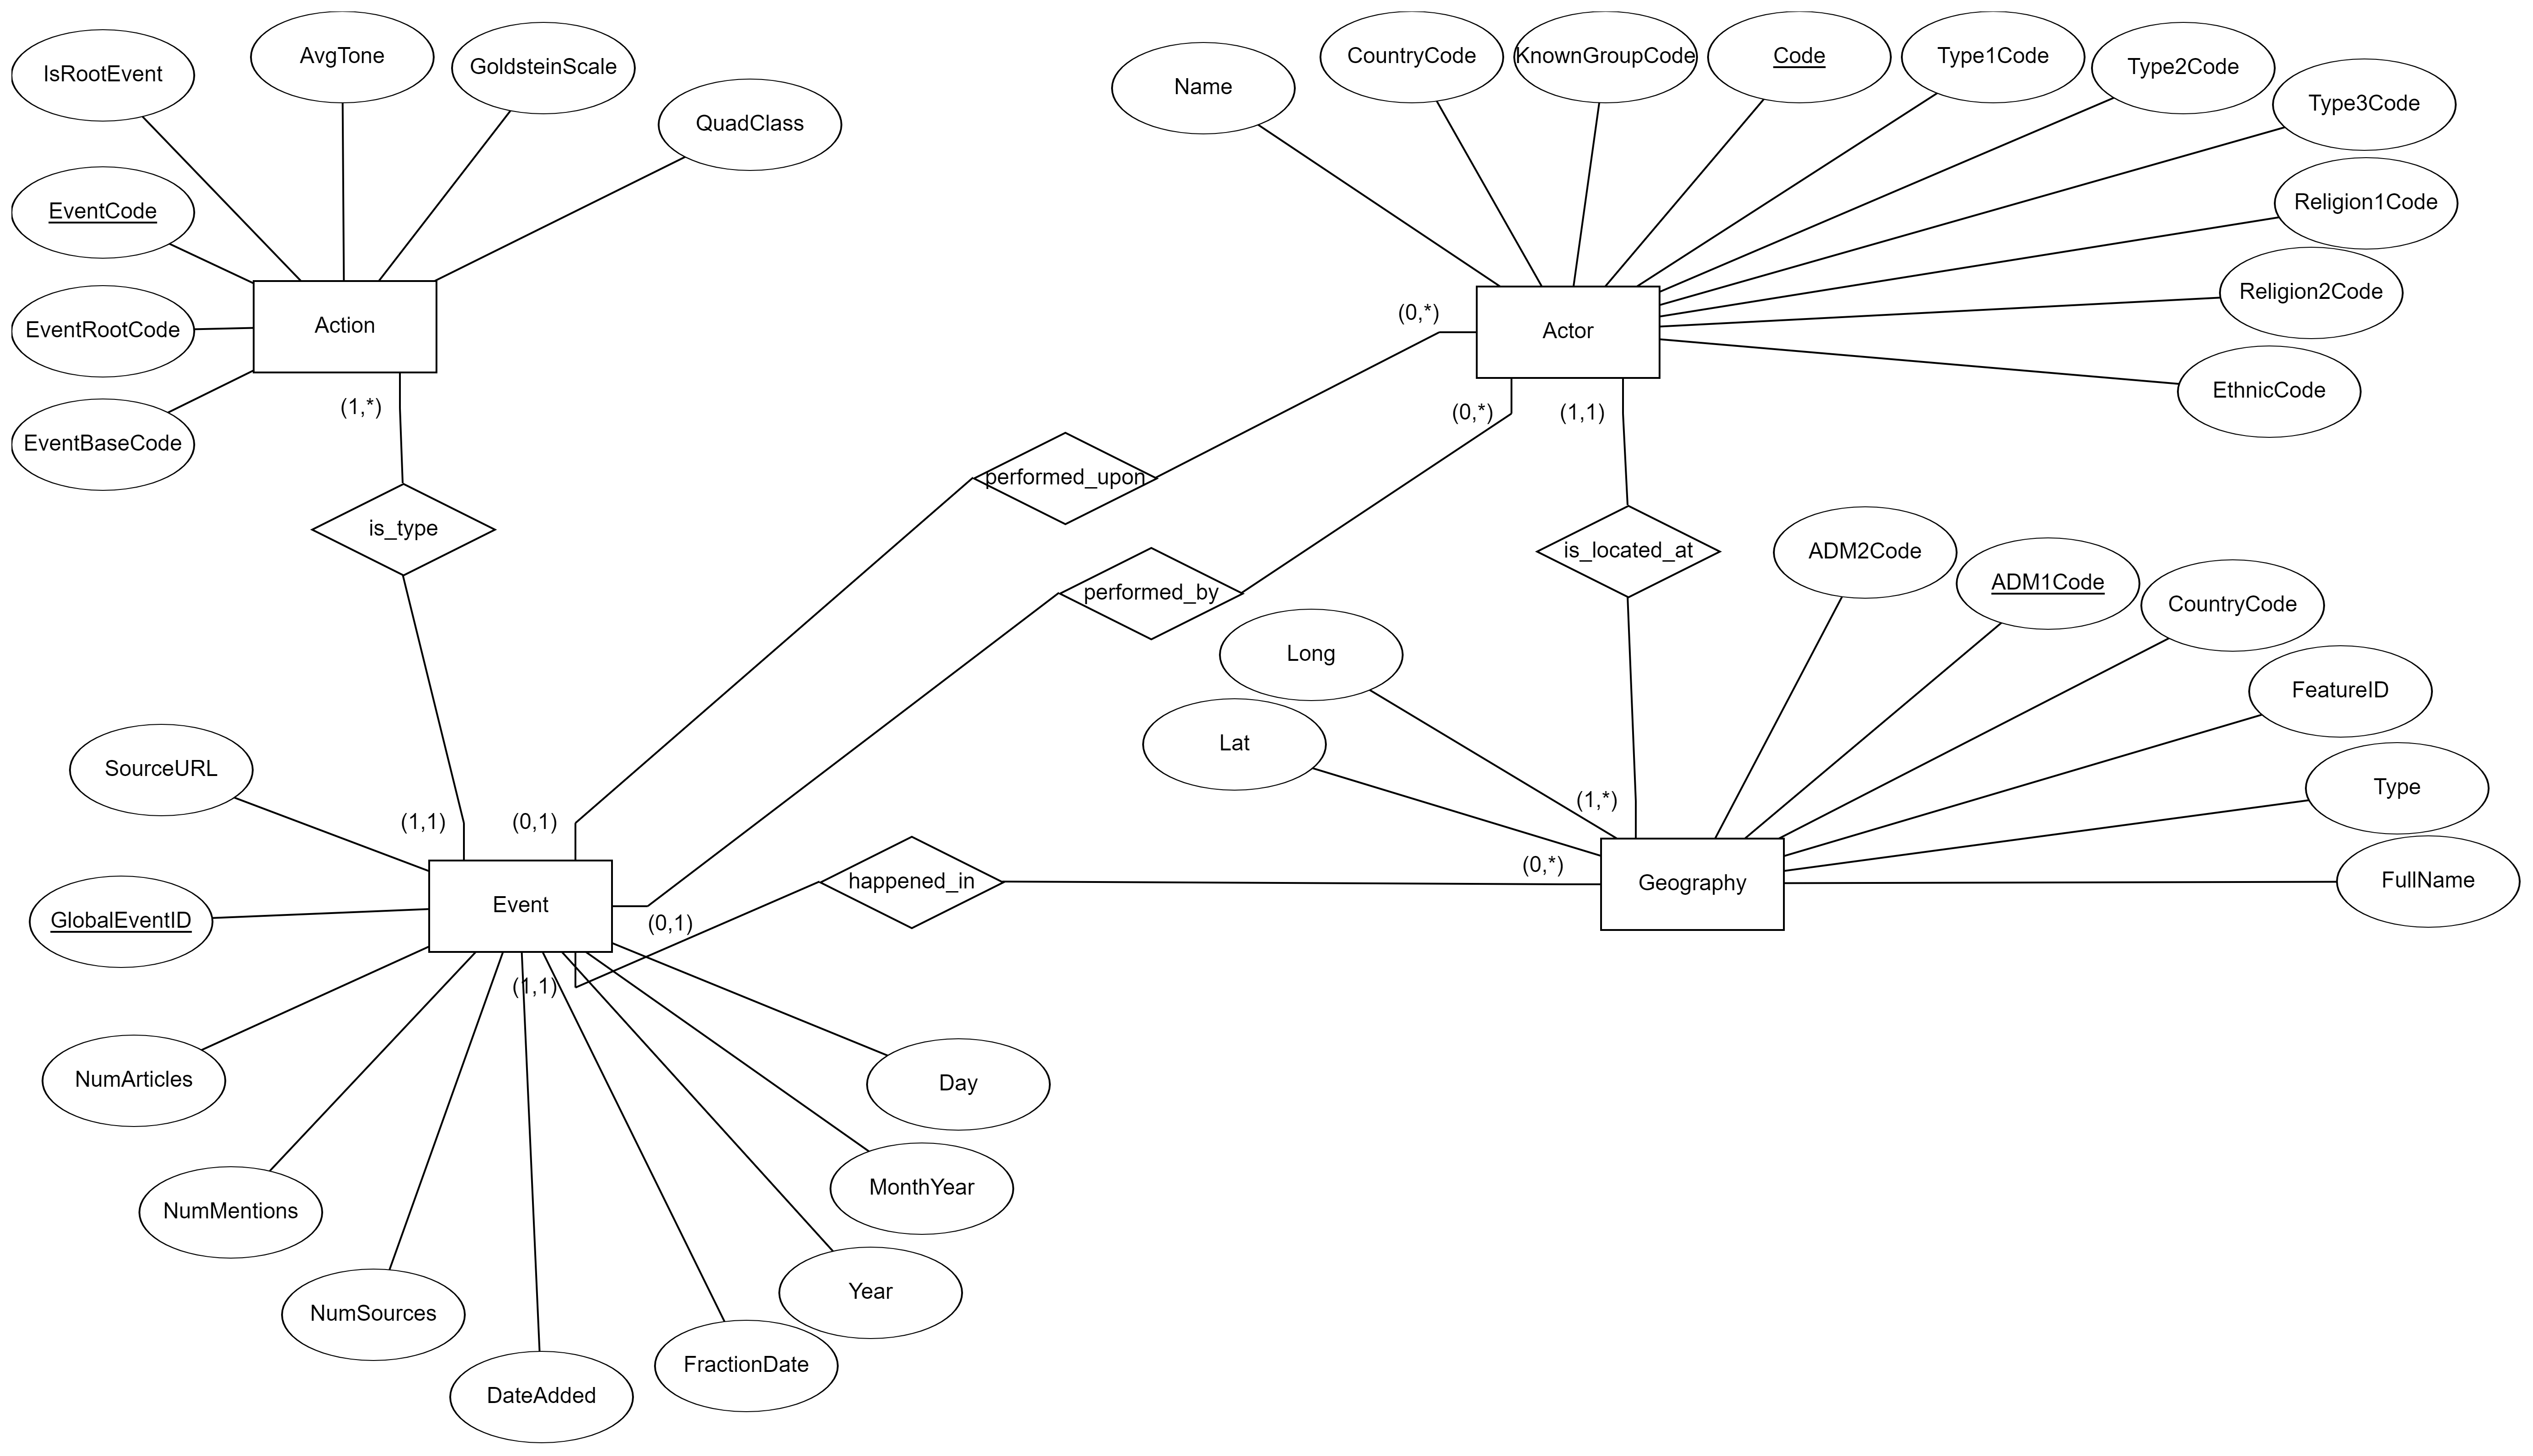
\includegraphics[scale = 0.08]{g9-gdelt}
	\caption{Our GDELT schema integration}
	\label{fig:gdelt}
\end{figure}

\begin{figure}
	\centering
	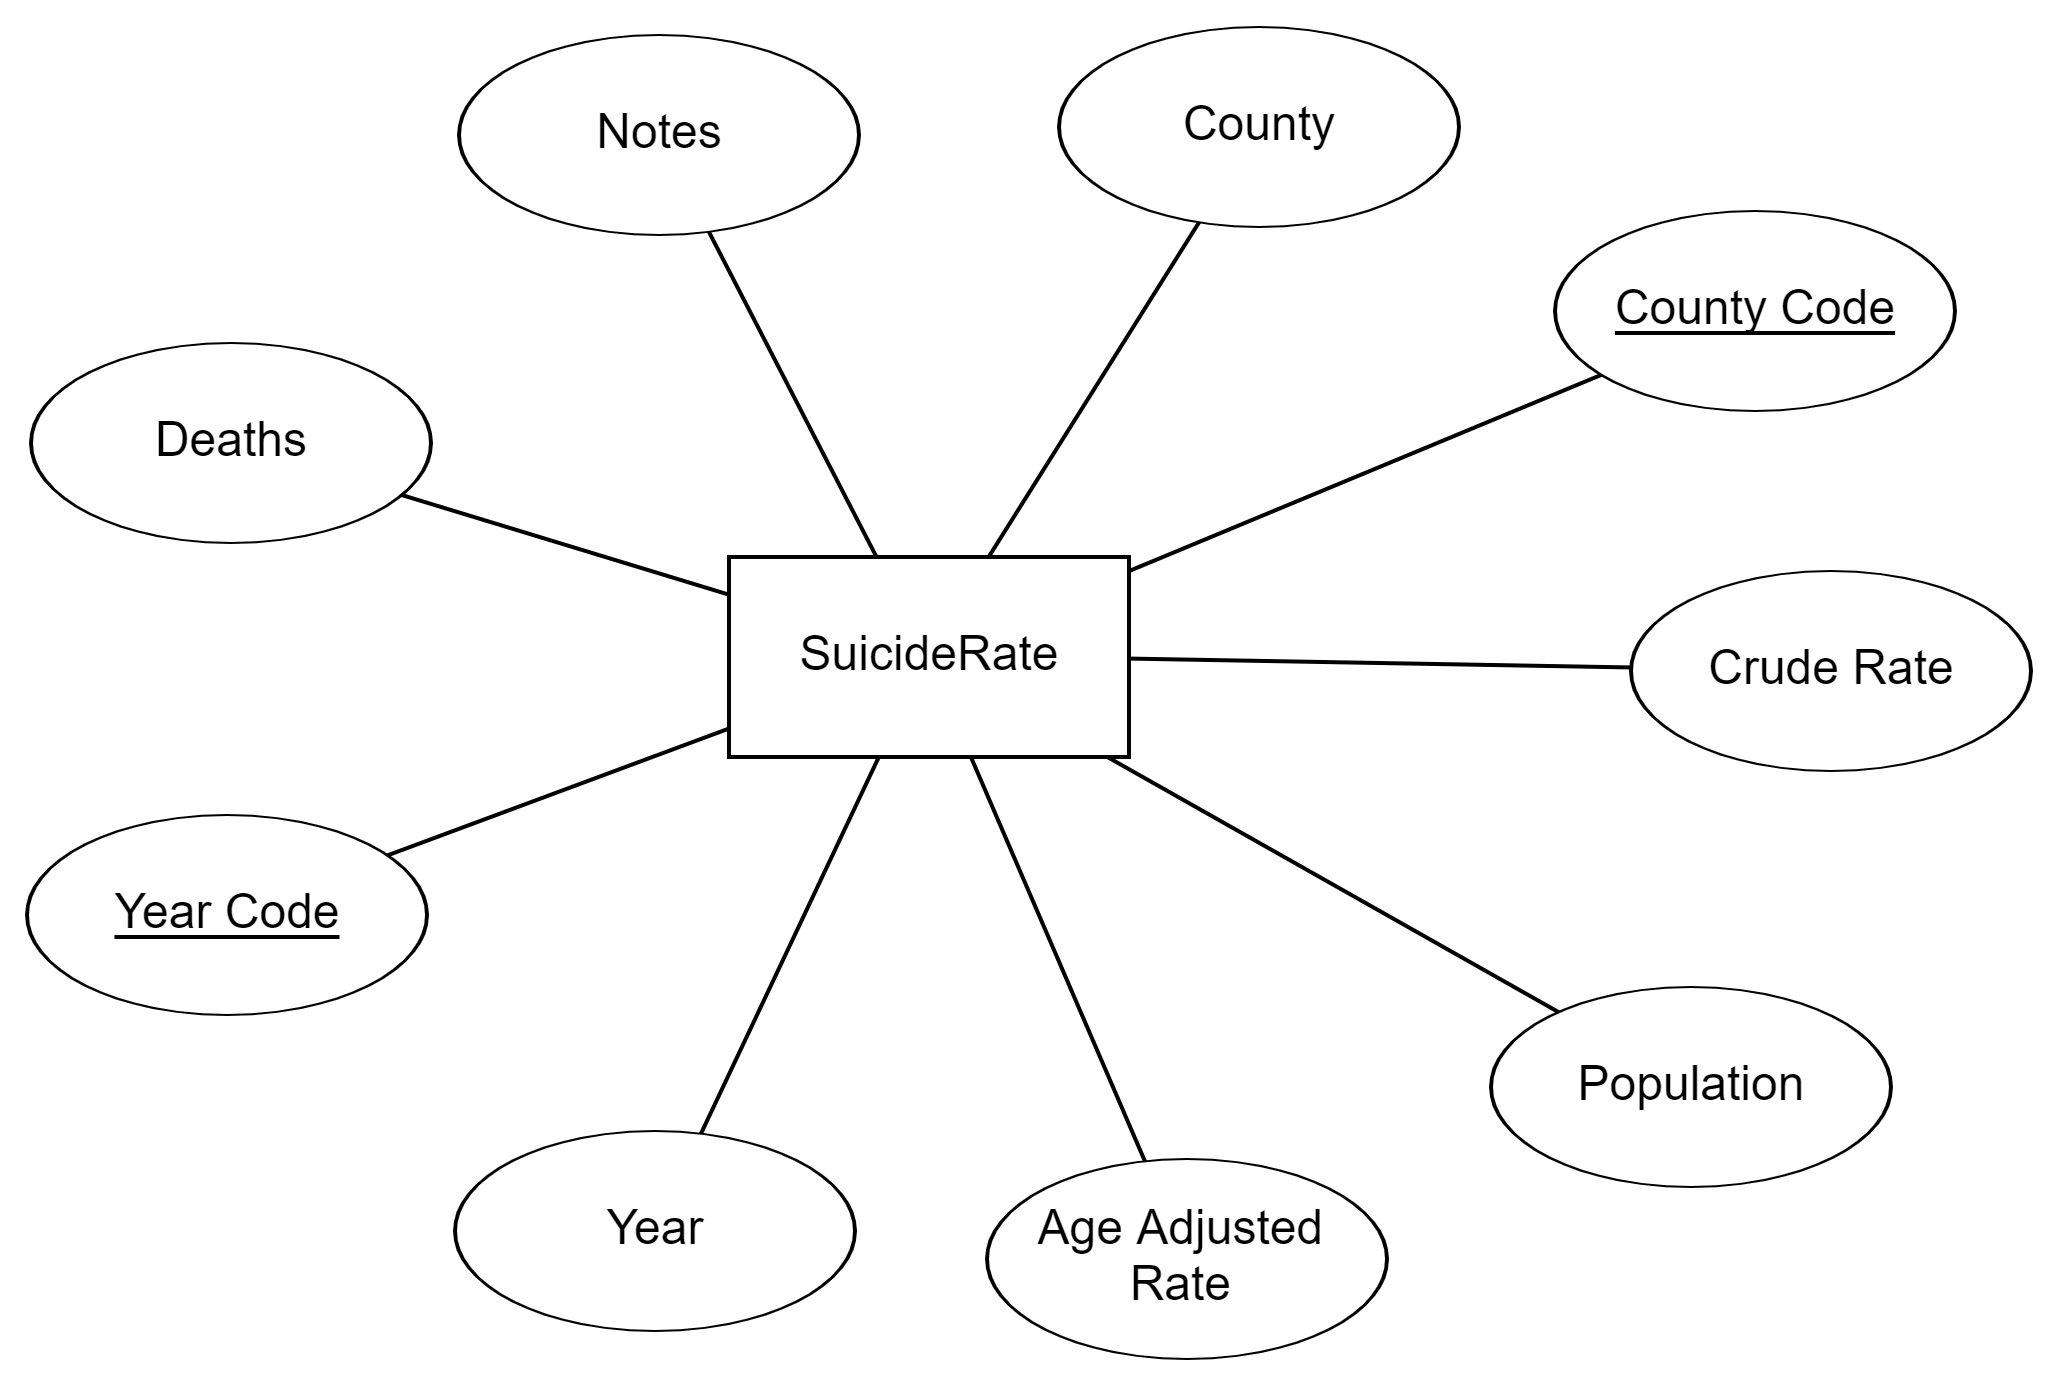
\includegraphics[scale = 0.18]{g9-suicide_rate}
	\caption{Our suicide rate schema integration}
	\label{fig:suicide_rate}
\end{figure}

\begin{figure}
	\centering
	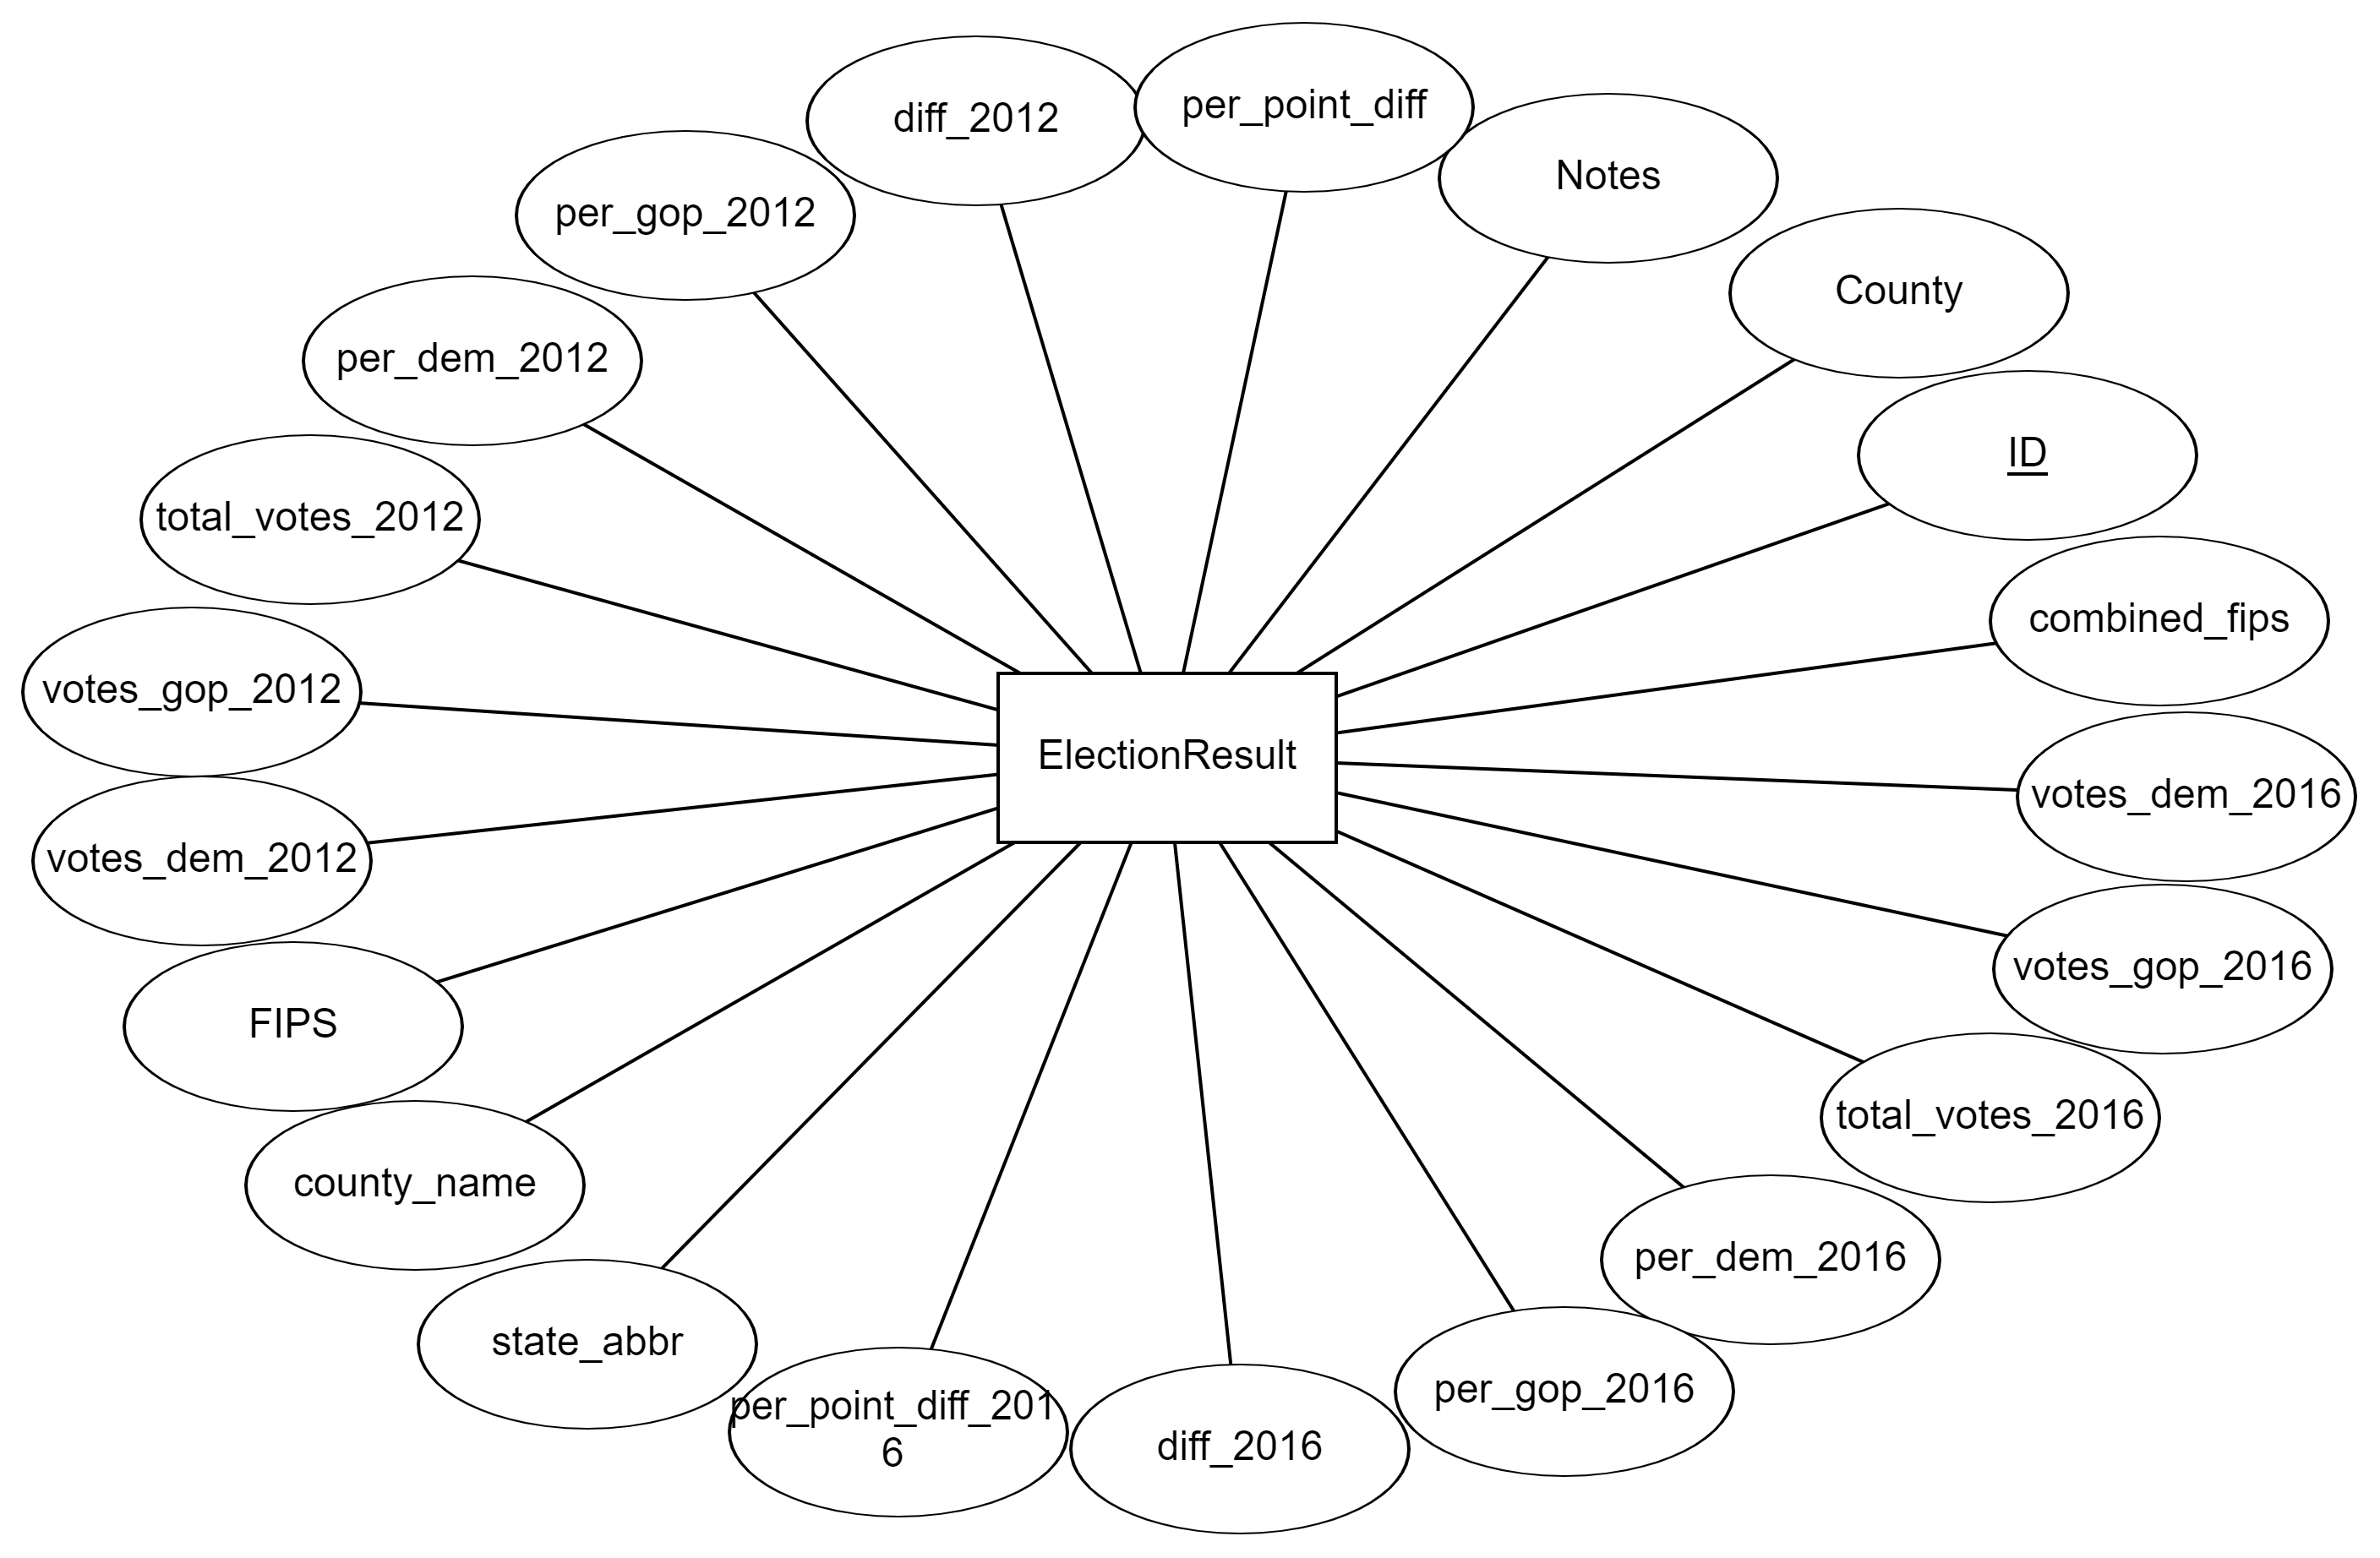
\includegraphics[scale = 0.12]{g9-election_results}
	\caption{Our election results integration}
	\label{fig:election_results}
\end{figure}

\begin{figure}
	\centering
	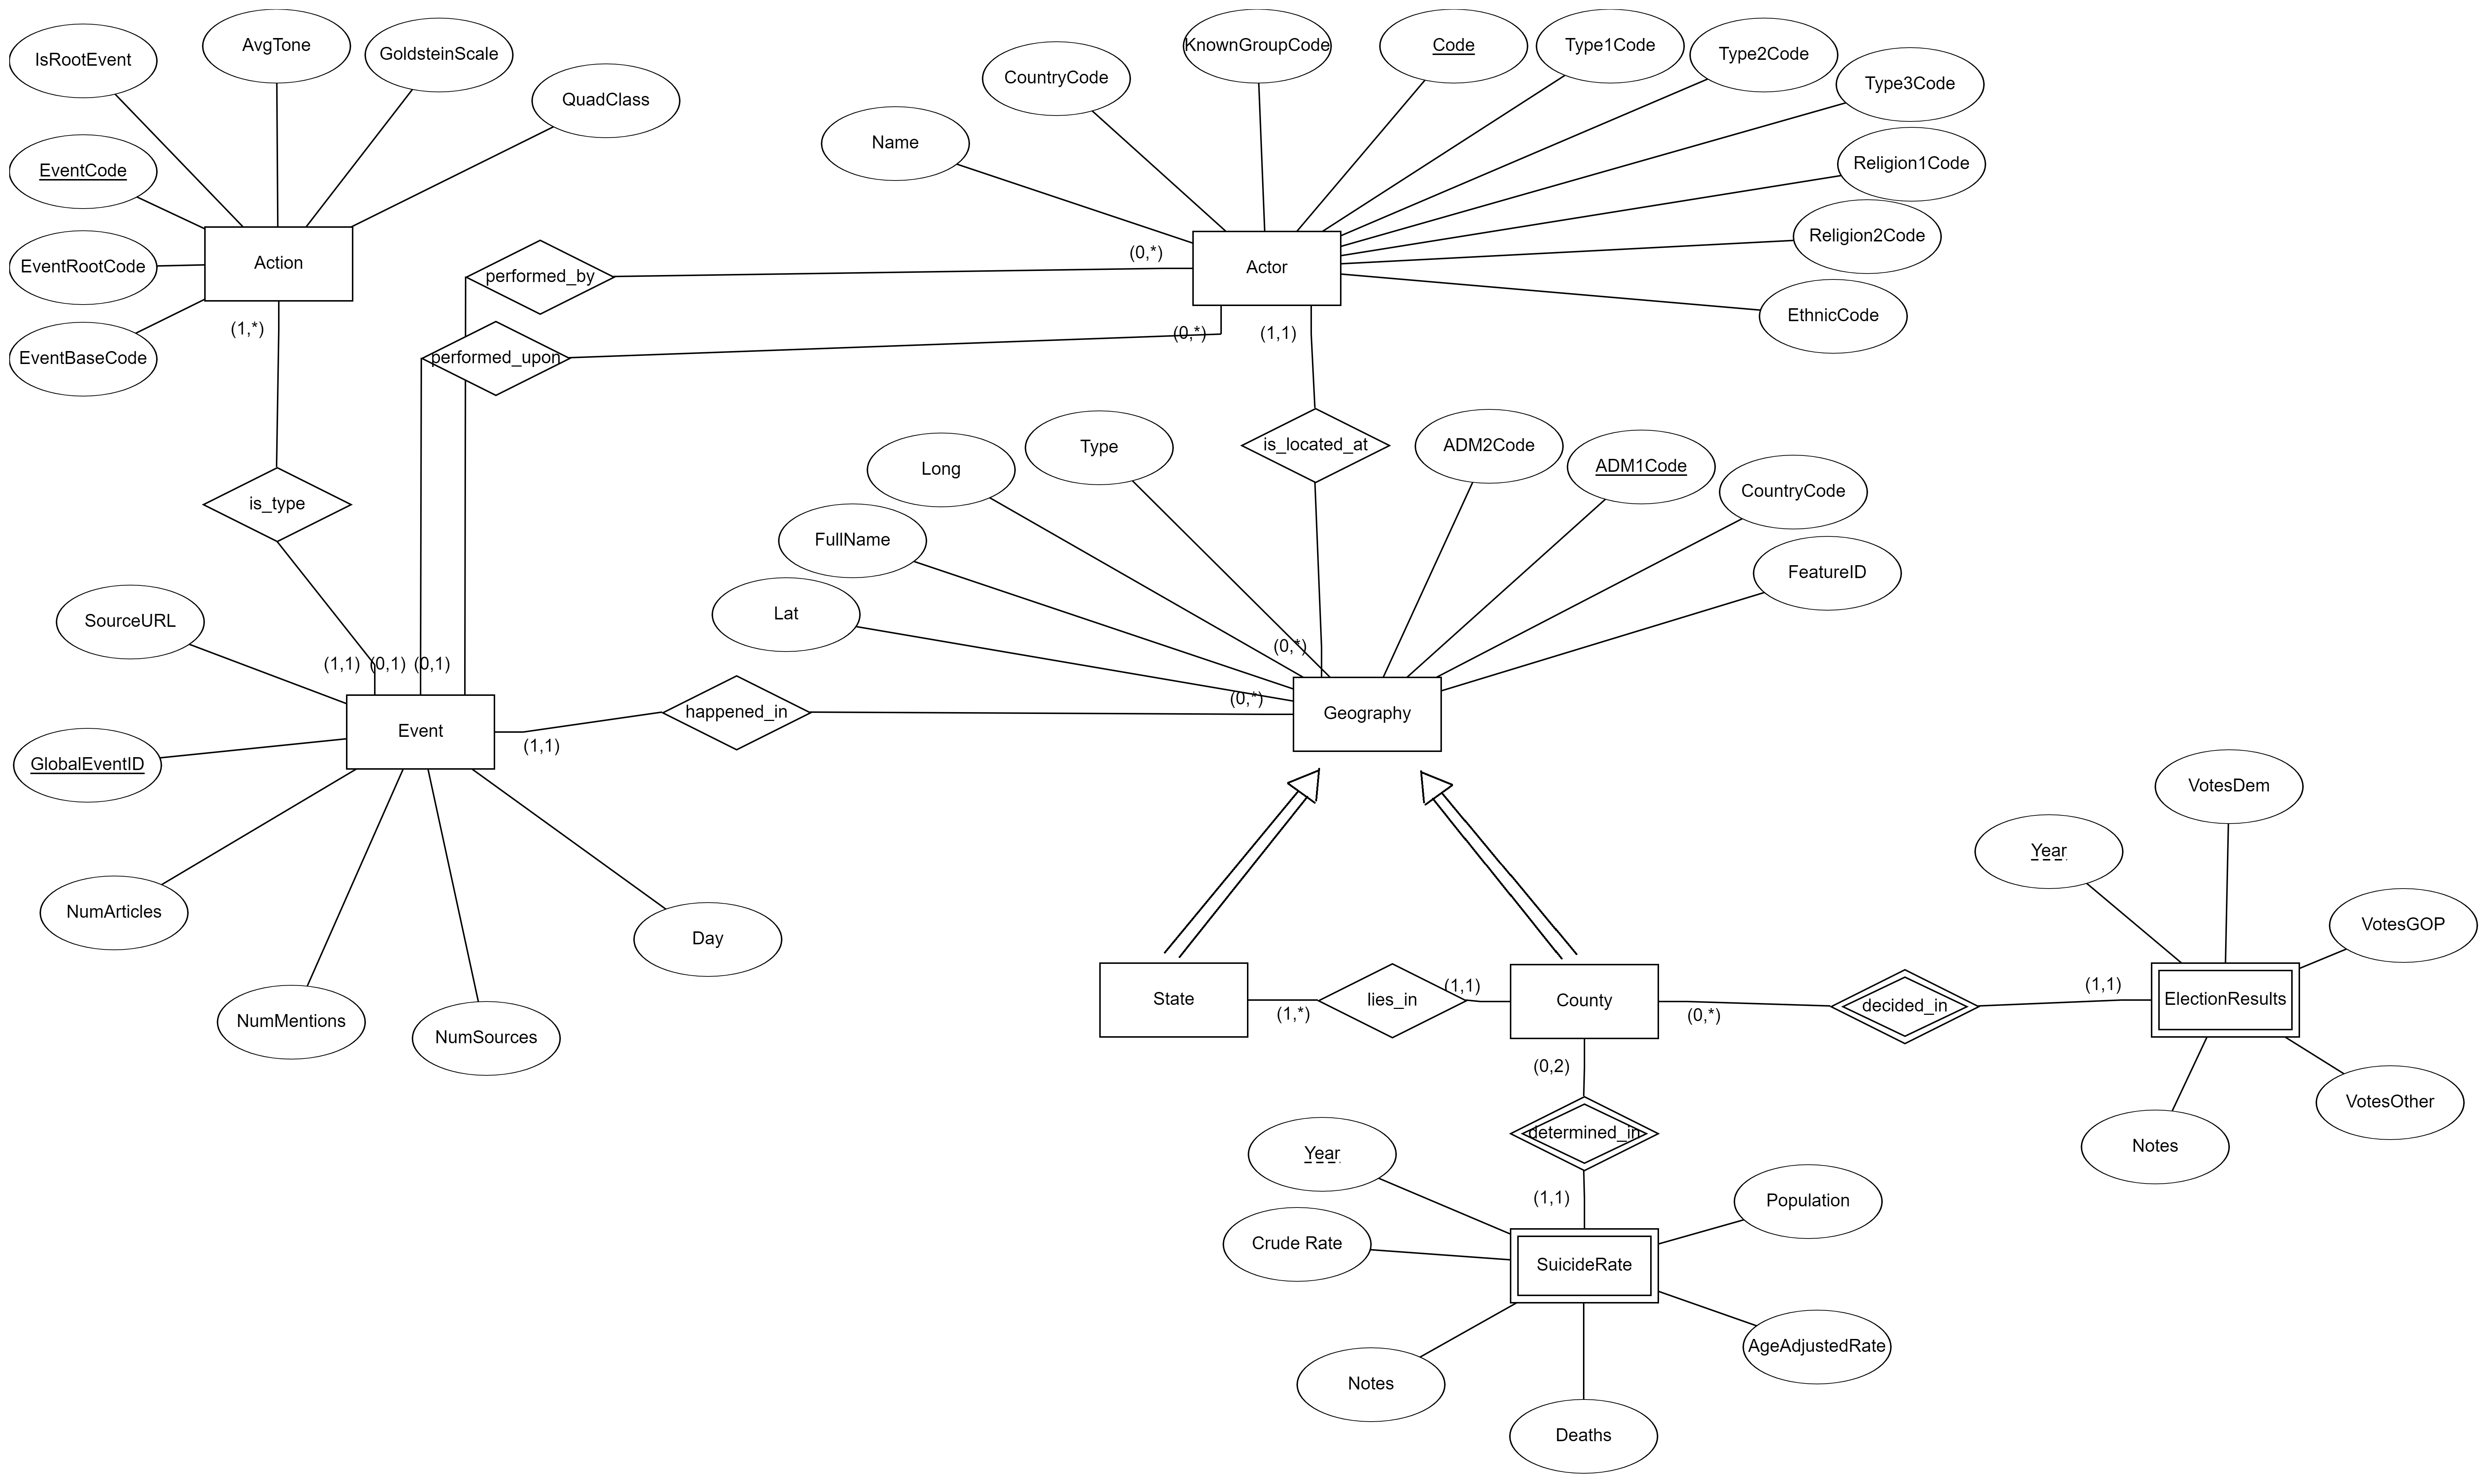
\includegraphics[scale = 0.08]{g9-all}
	\caption{Schema over the whole database}
	\label{fig:all}
\end{figure}


\textbf{Putting it all together}:
The election results and the Suicide Rate data sets have the
county attribute in common.
A county lies in a state, and both a county and a state are
spesializations of a "geography".
Some other attributes can be removed since they are redundant
(e.g. MonthYear makes the Year attribute irrelevant).
The end result can be seen on figure \ref{fig:all}.

\textbf{Technical parts}
On the inegration process, we tried using the counties' FIPS codes
present on each of the datasets to link the different entities
together.
However we quickly learned that each dataset's FIPS code
contradicts the FIPS code each other data set.

Our solution has been to identify each county (and state)
by a geoID code than can be derived from {\color{red}{todo
https://community.esri.com/thread/24614
ESRI
}}.

The only other hazard occurs when ElectionResults generates an
ID that does not match any County, in that case the corresponding
row is simply skipped and also printed to STDOUT for reference.

%The GDELT data subset we use in this project consists of sixty
three thousand csv files, where each file takes somewhere between
800 KB and 1.5 MB of storage.

On our P2 hand-in we include a script
(/gdelt/download.py) that downloads each csv file
and edits the filenames for further processing.
If a file is found to be corrupt, it is not downloaded and
the index of the file is saved in a .txt file
(/gdelt/bad\_indices.txt).

The dataset consists of sixty attributes and the domain of
each attribute is in detail on the official handbook
{\color{red}{citation}}.

Moving on, the suicide rate dataset can be obtained from
the Centers for Disease Control and Prevention
website \cite{suicide_website}.

The election results dataset is straightforward, it can be
obtained on {\color{red}{todo}}.

\begin{figure}
	\centering
	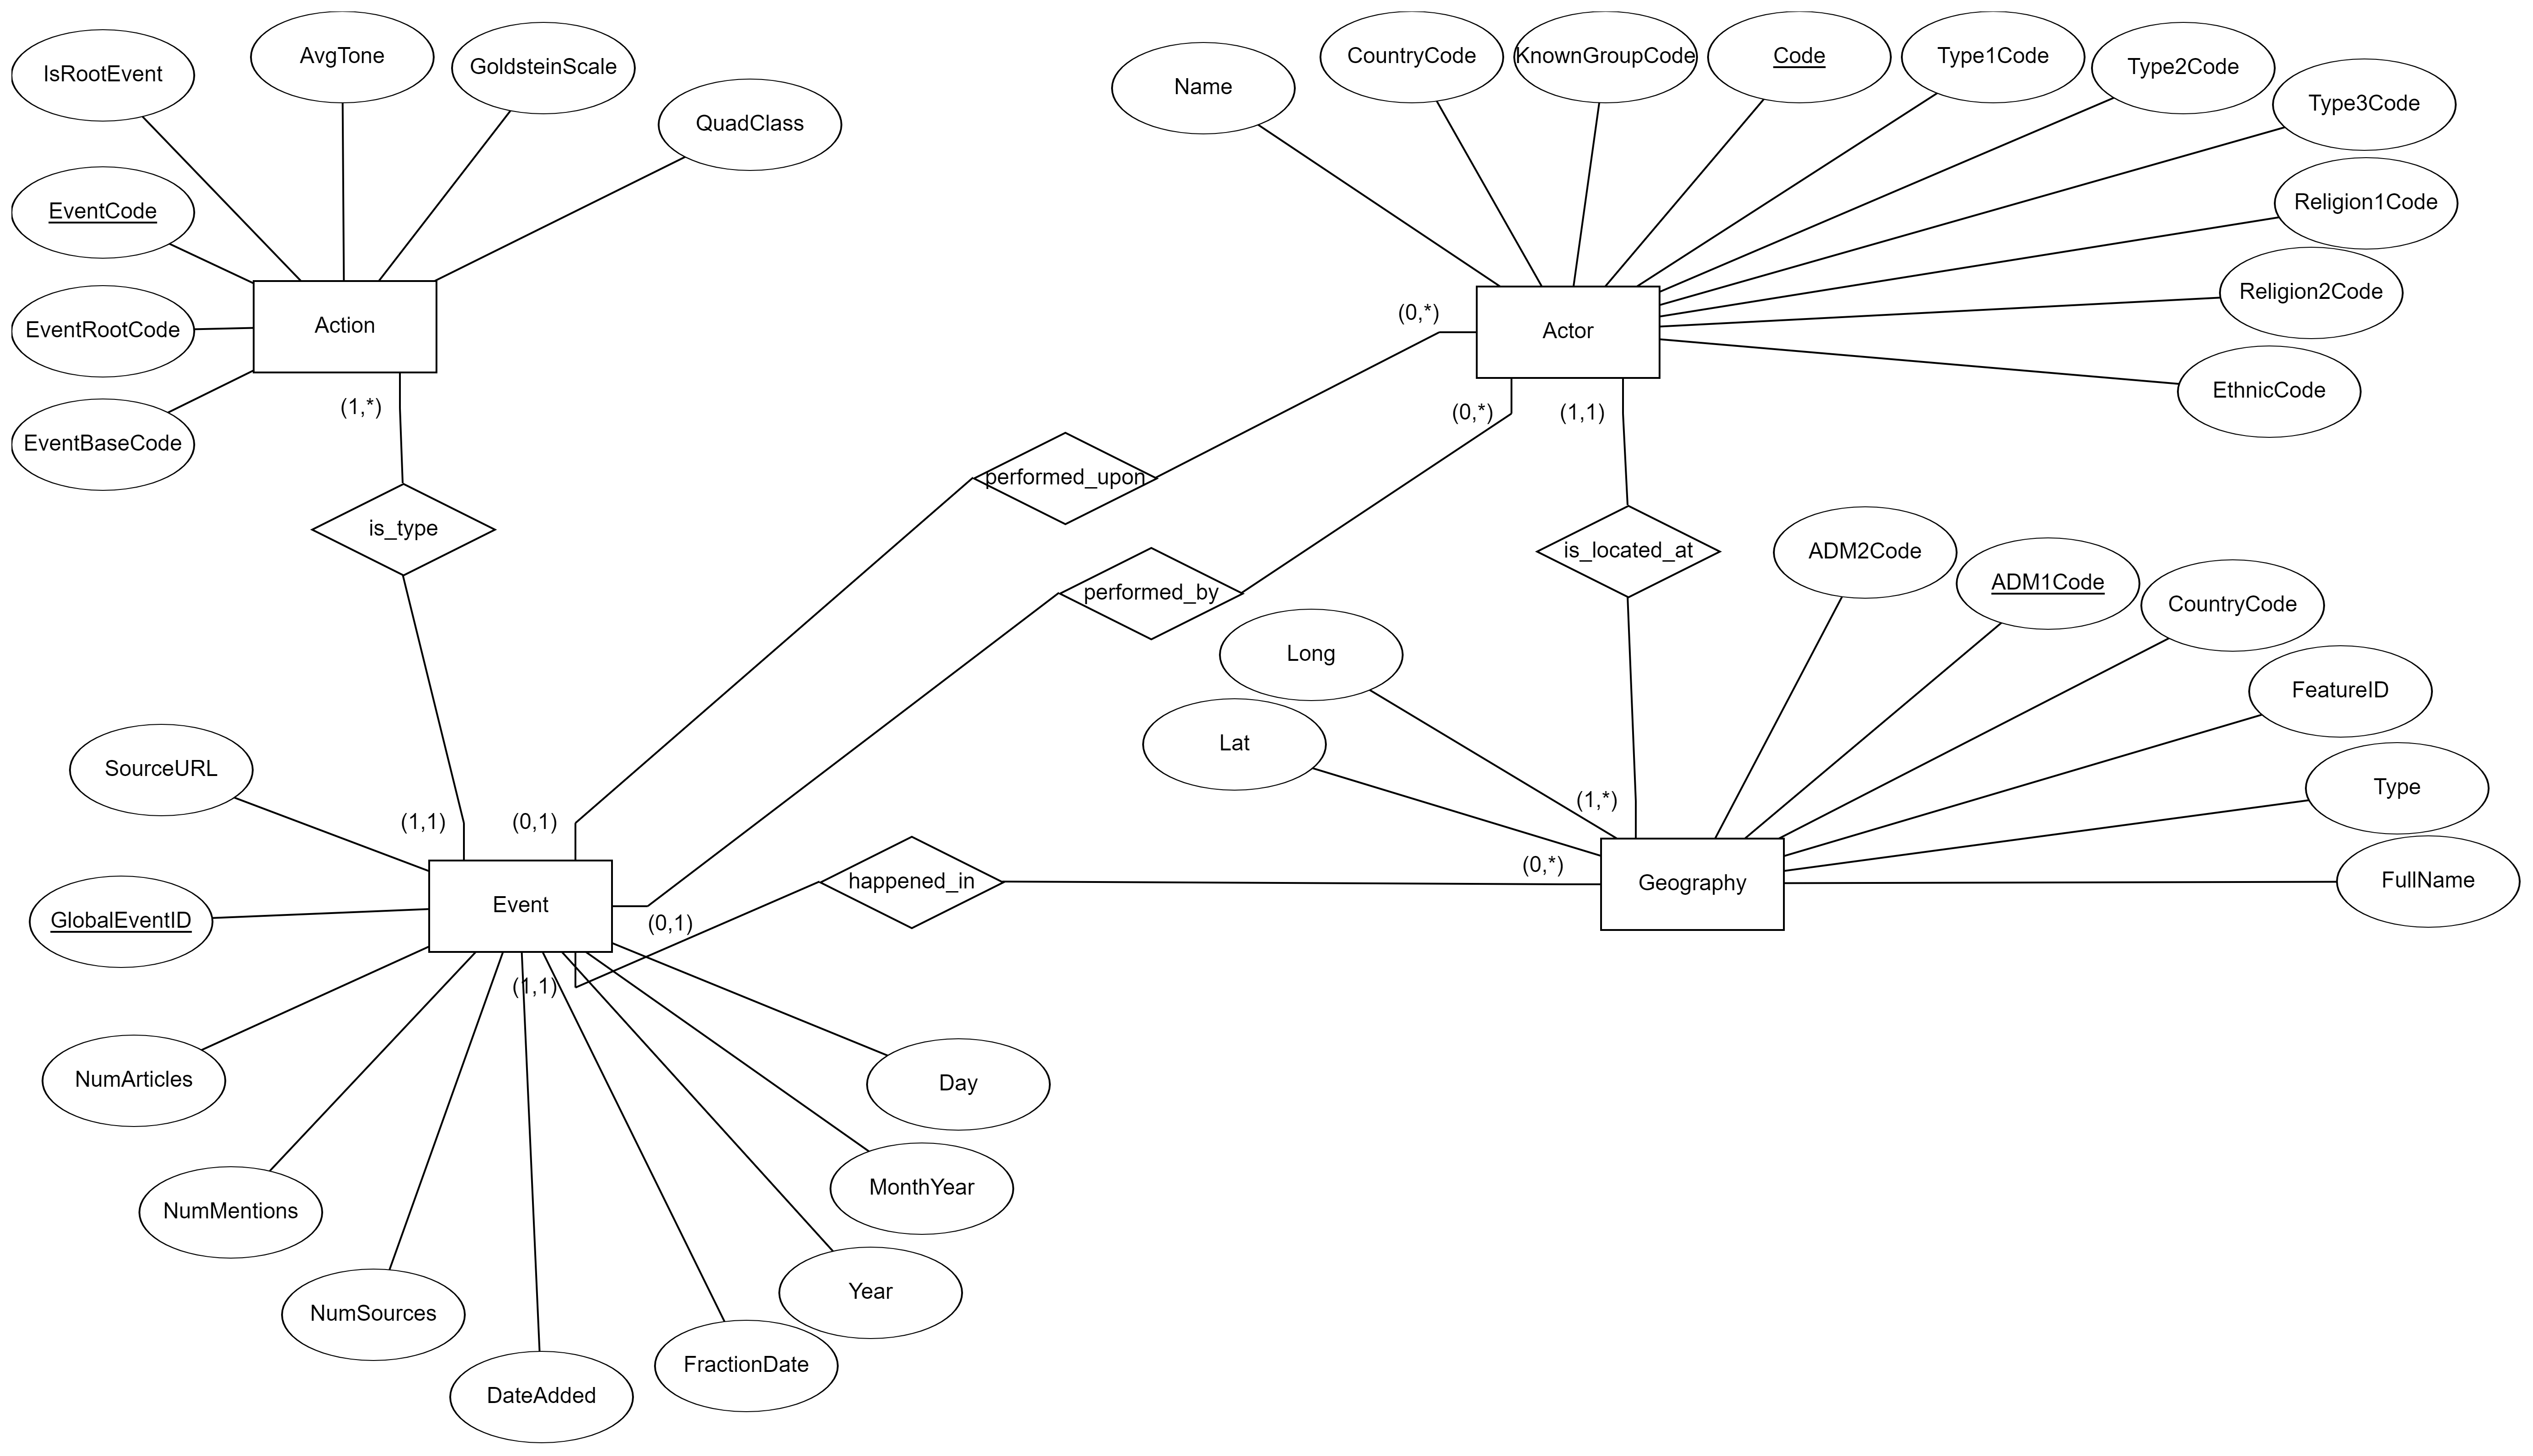
\includegraphics[scale = 0.08]{g9-gdelt}
	\caption{Our GDELT schema integration}
	\label{fig:gdelt}
\end{figure}

\begin{figure}
	\centering
	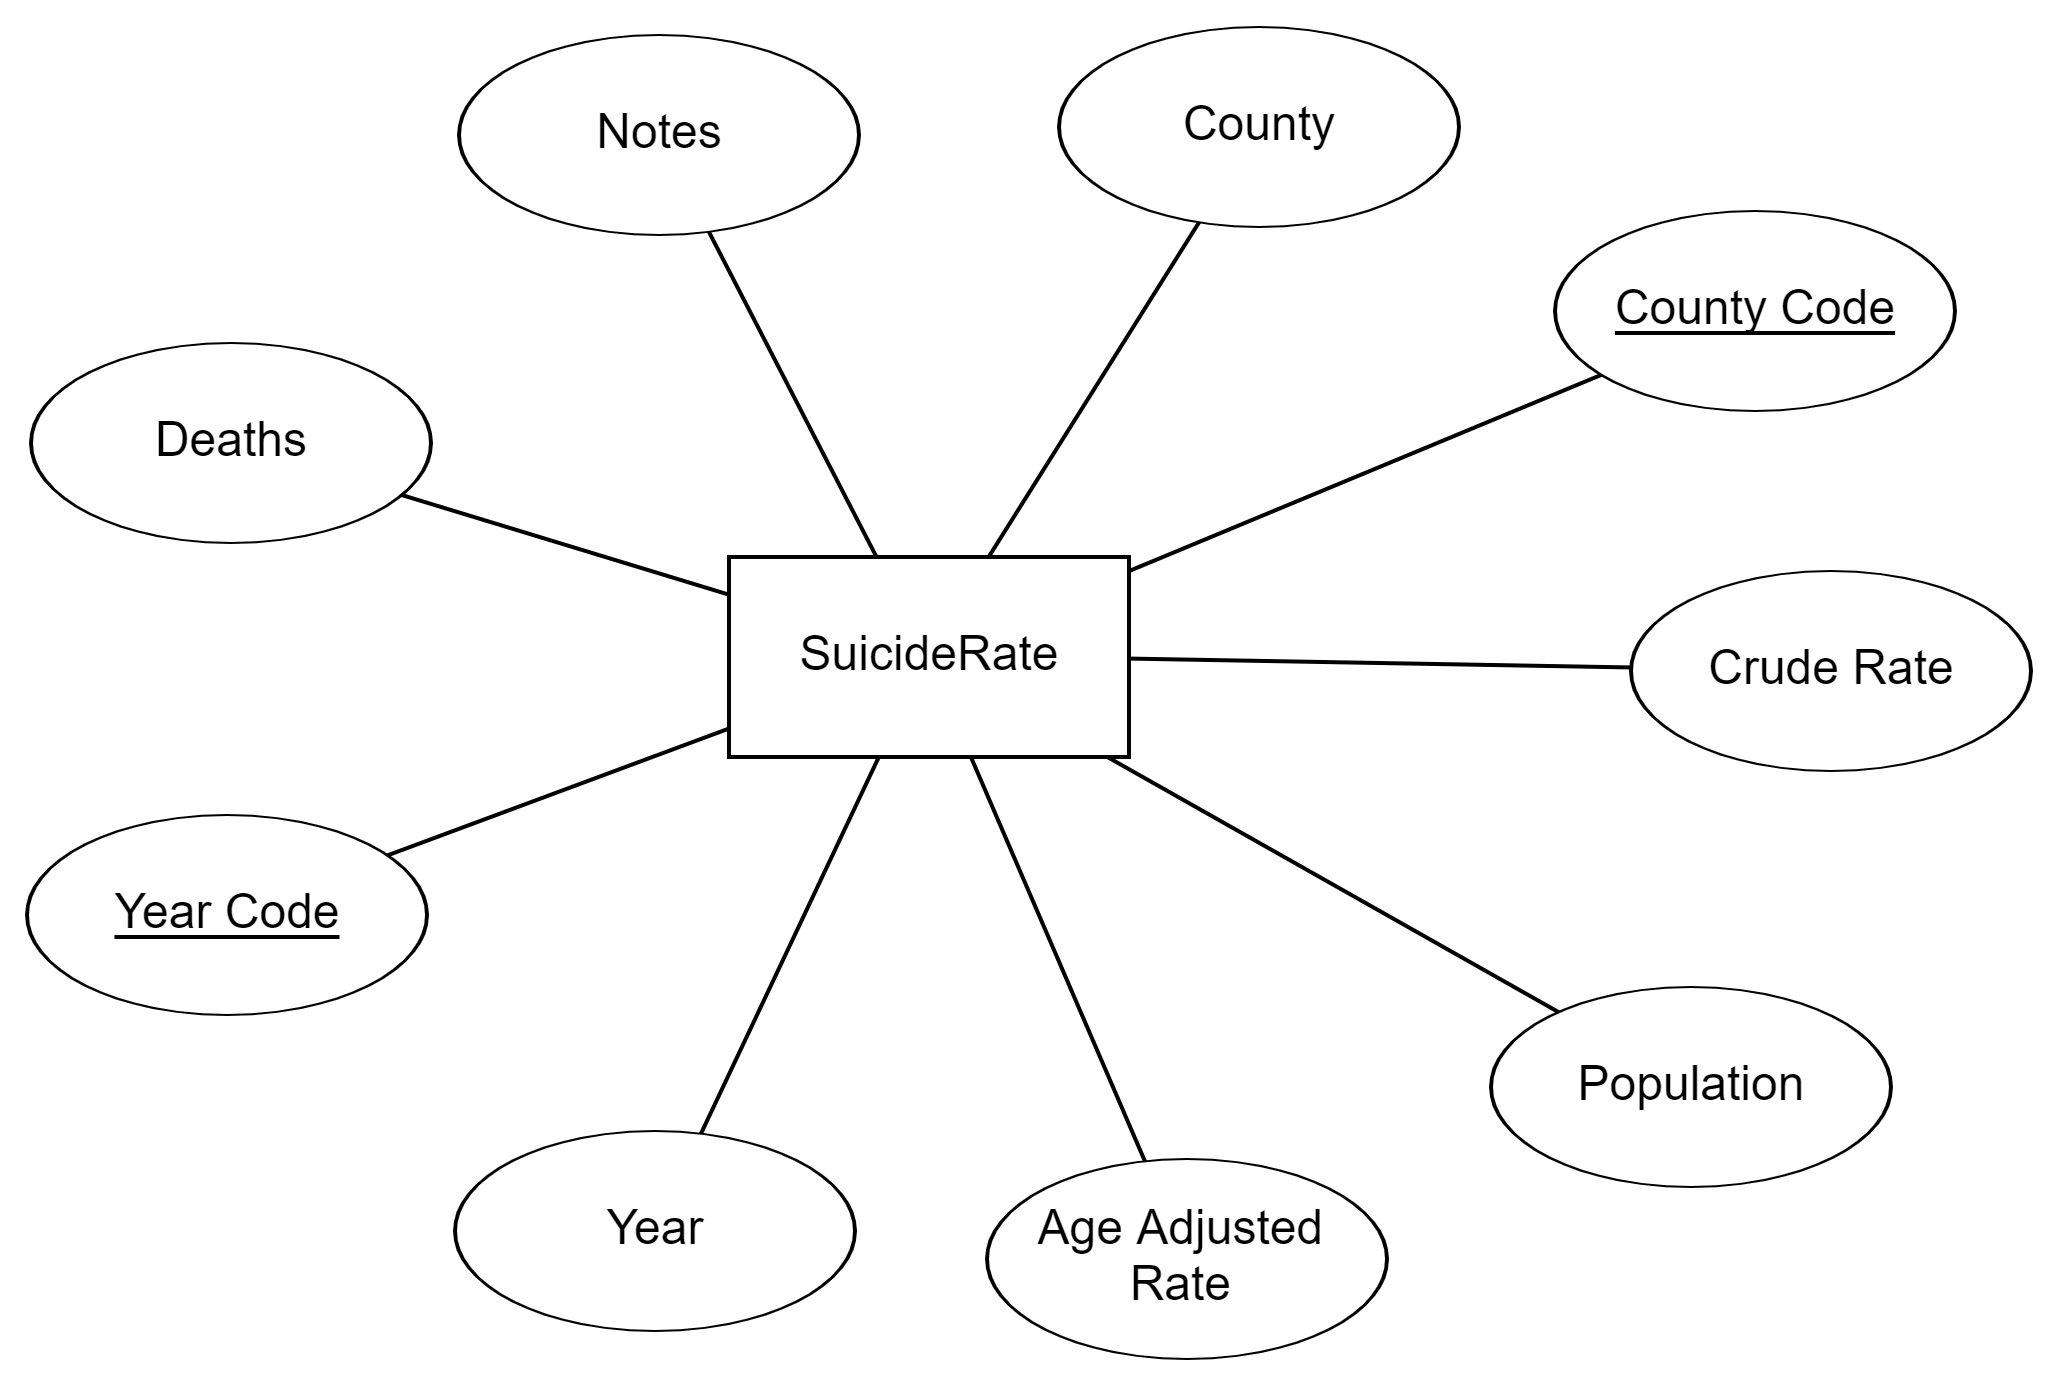
\includegraphics[scale = 0.18]{g9-suicide_rate}
	\caption{Our suicide rate schema integration}
	\label{fig:suicide_rate}
\end{figure}

\begin{figure}
	\centering
	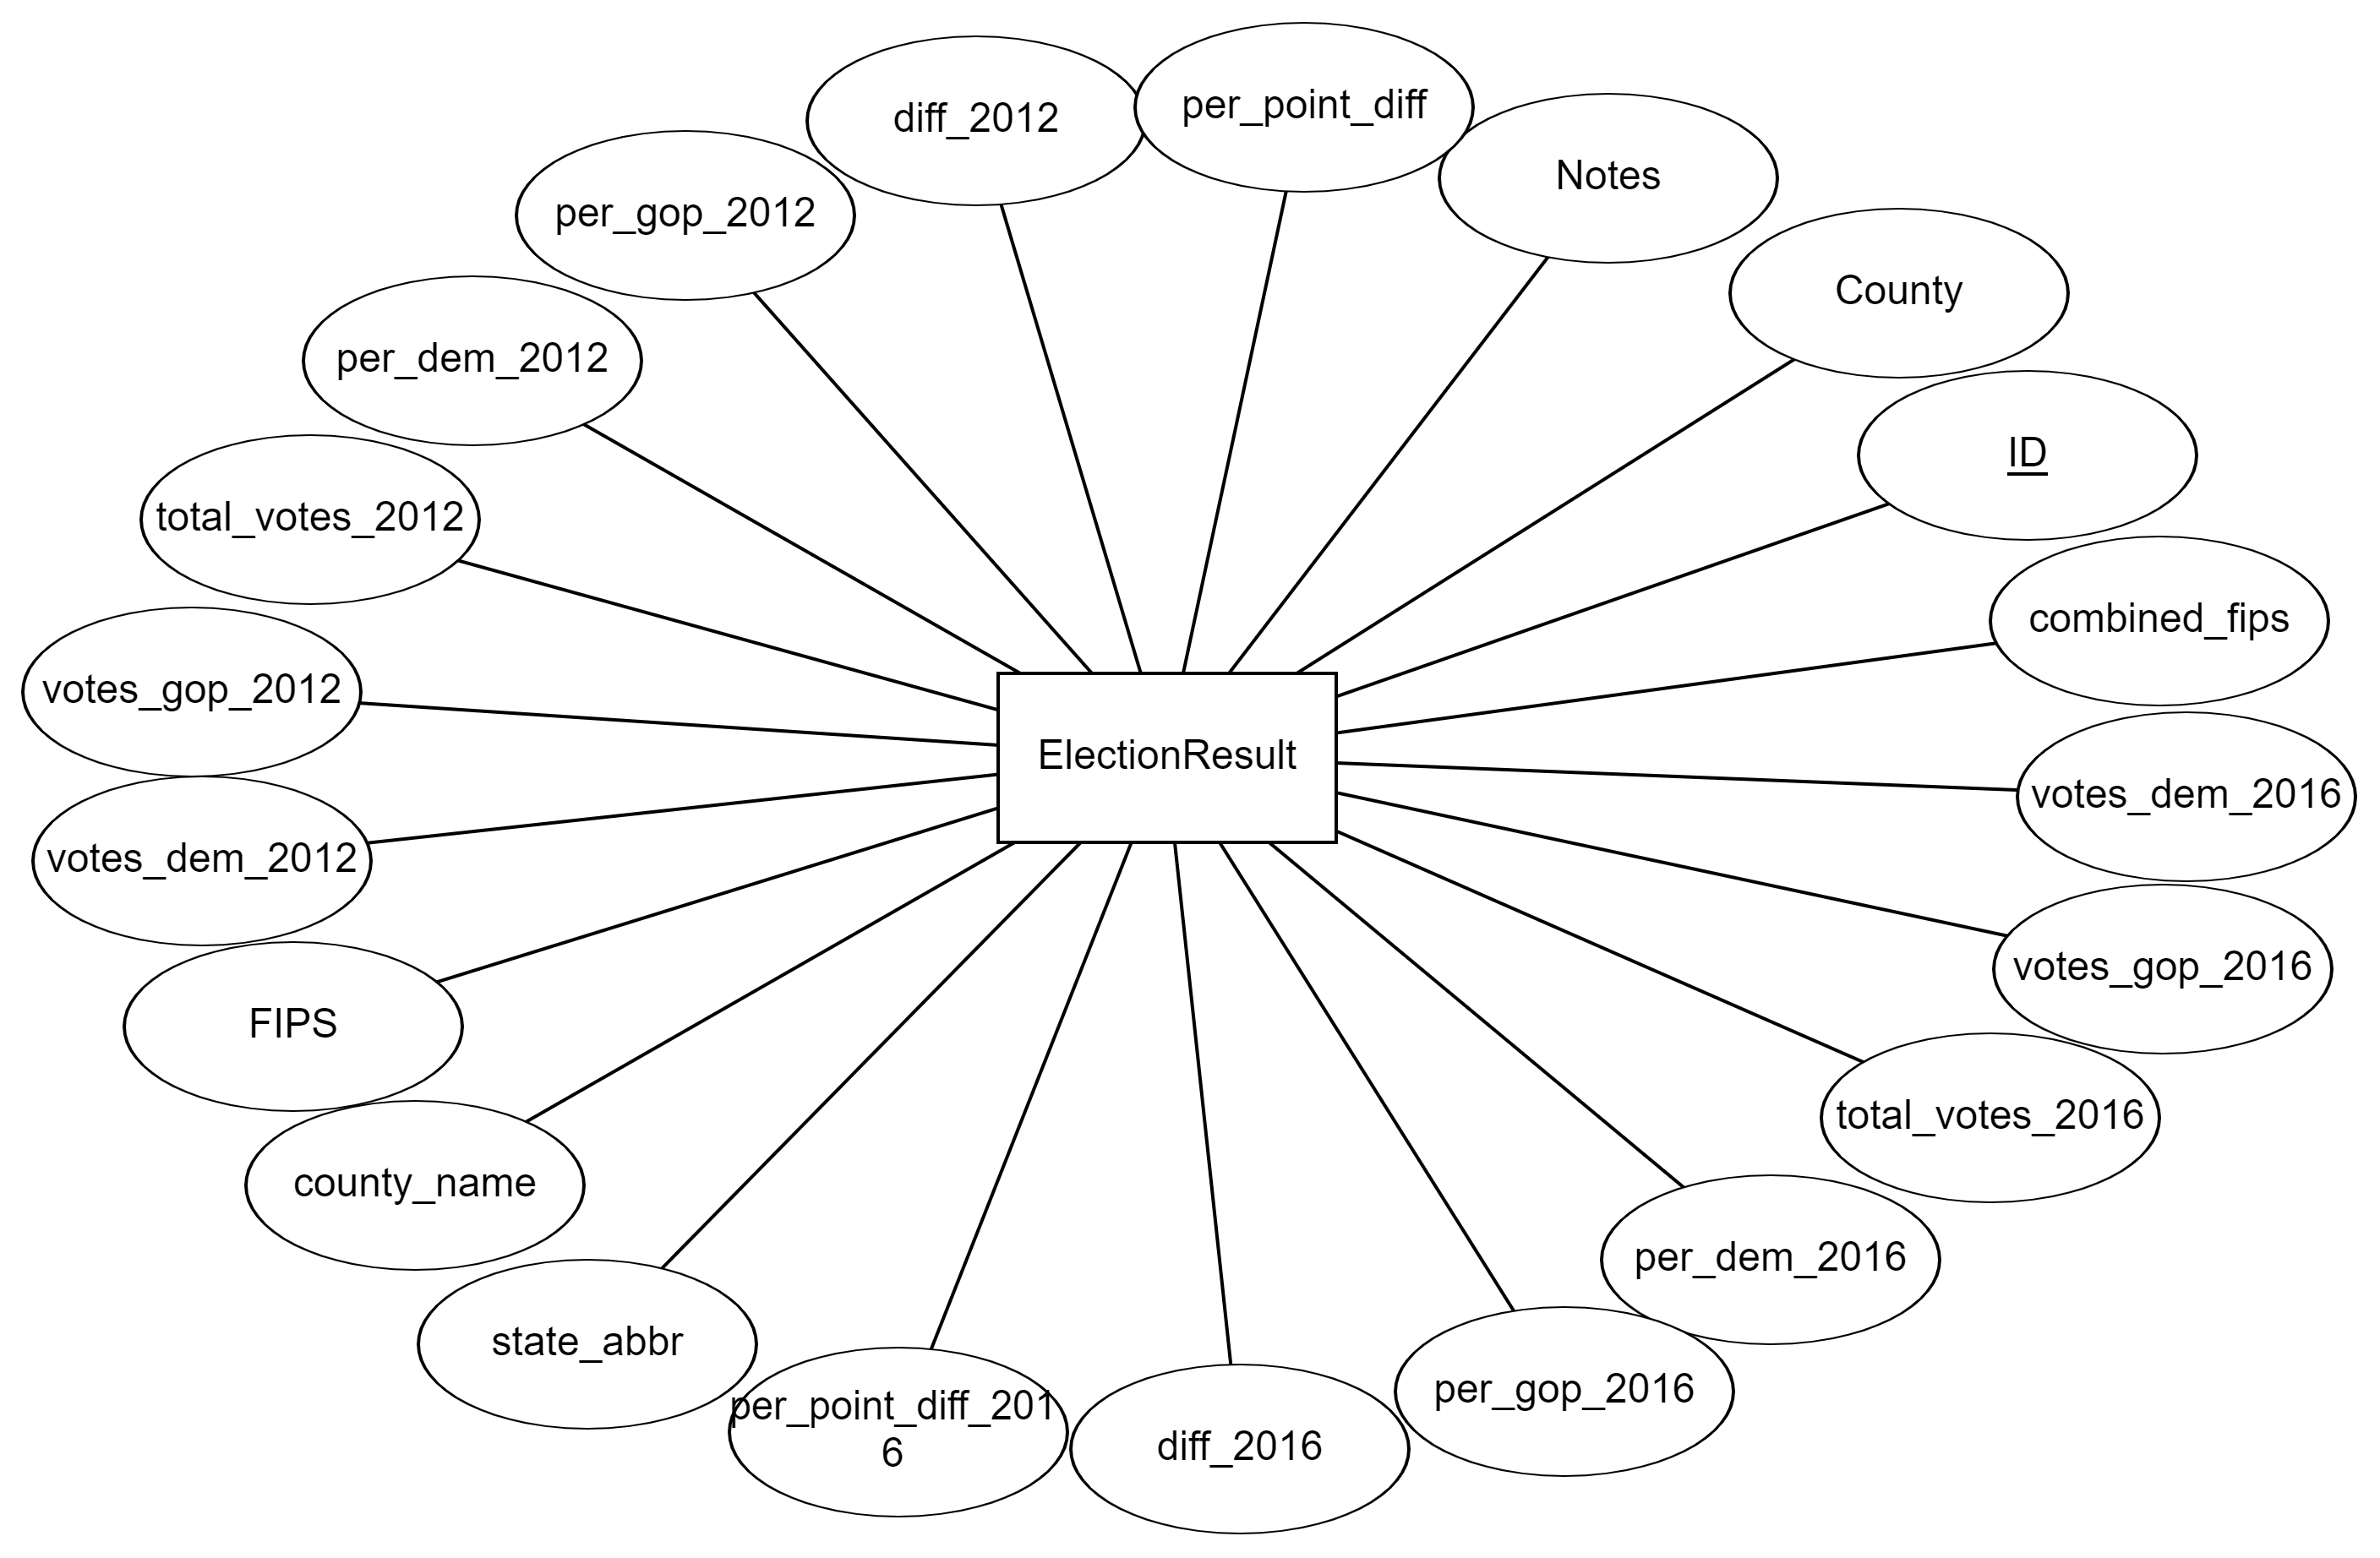
\includegraphics[scale = 0.12]{g9-election_results}
	\caption{Our election results integration}
	\label{fig:election_results}
\end{figure}

\begin{figure}
	\centering
	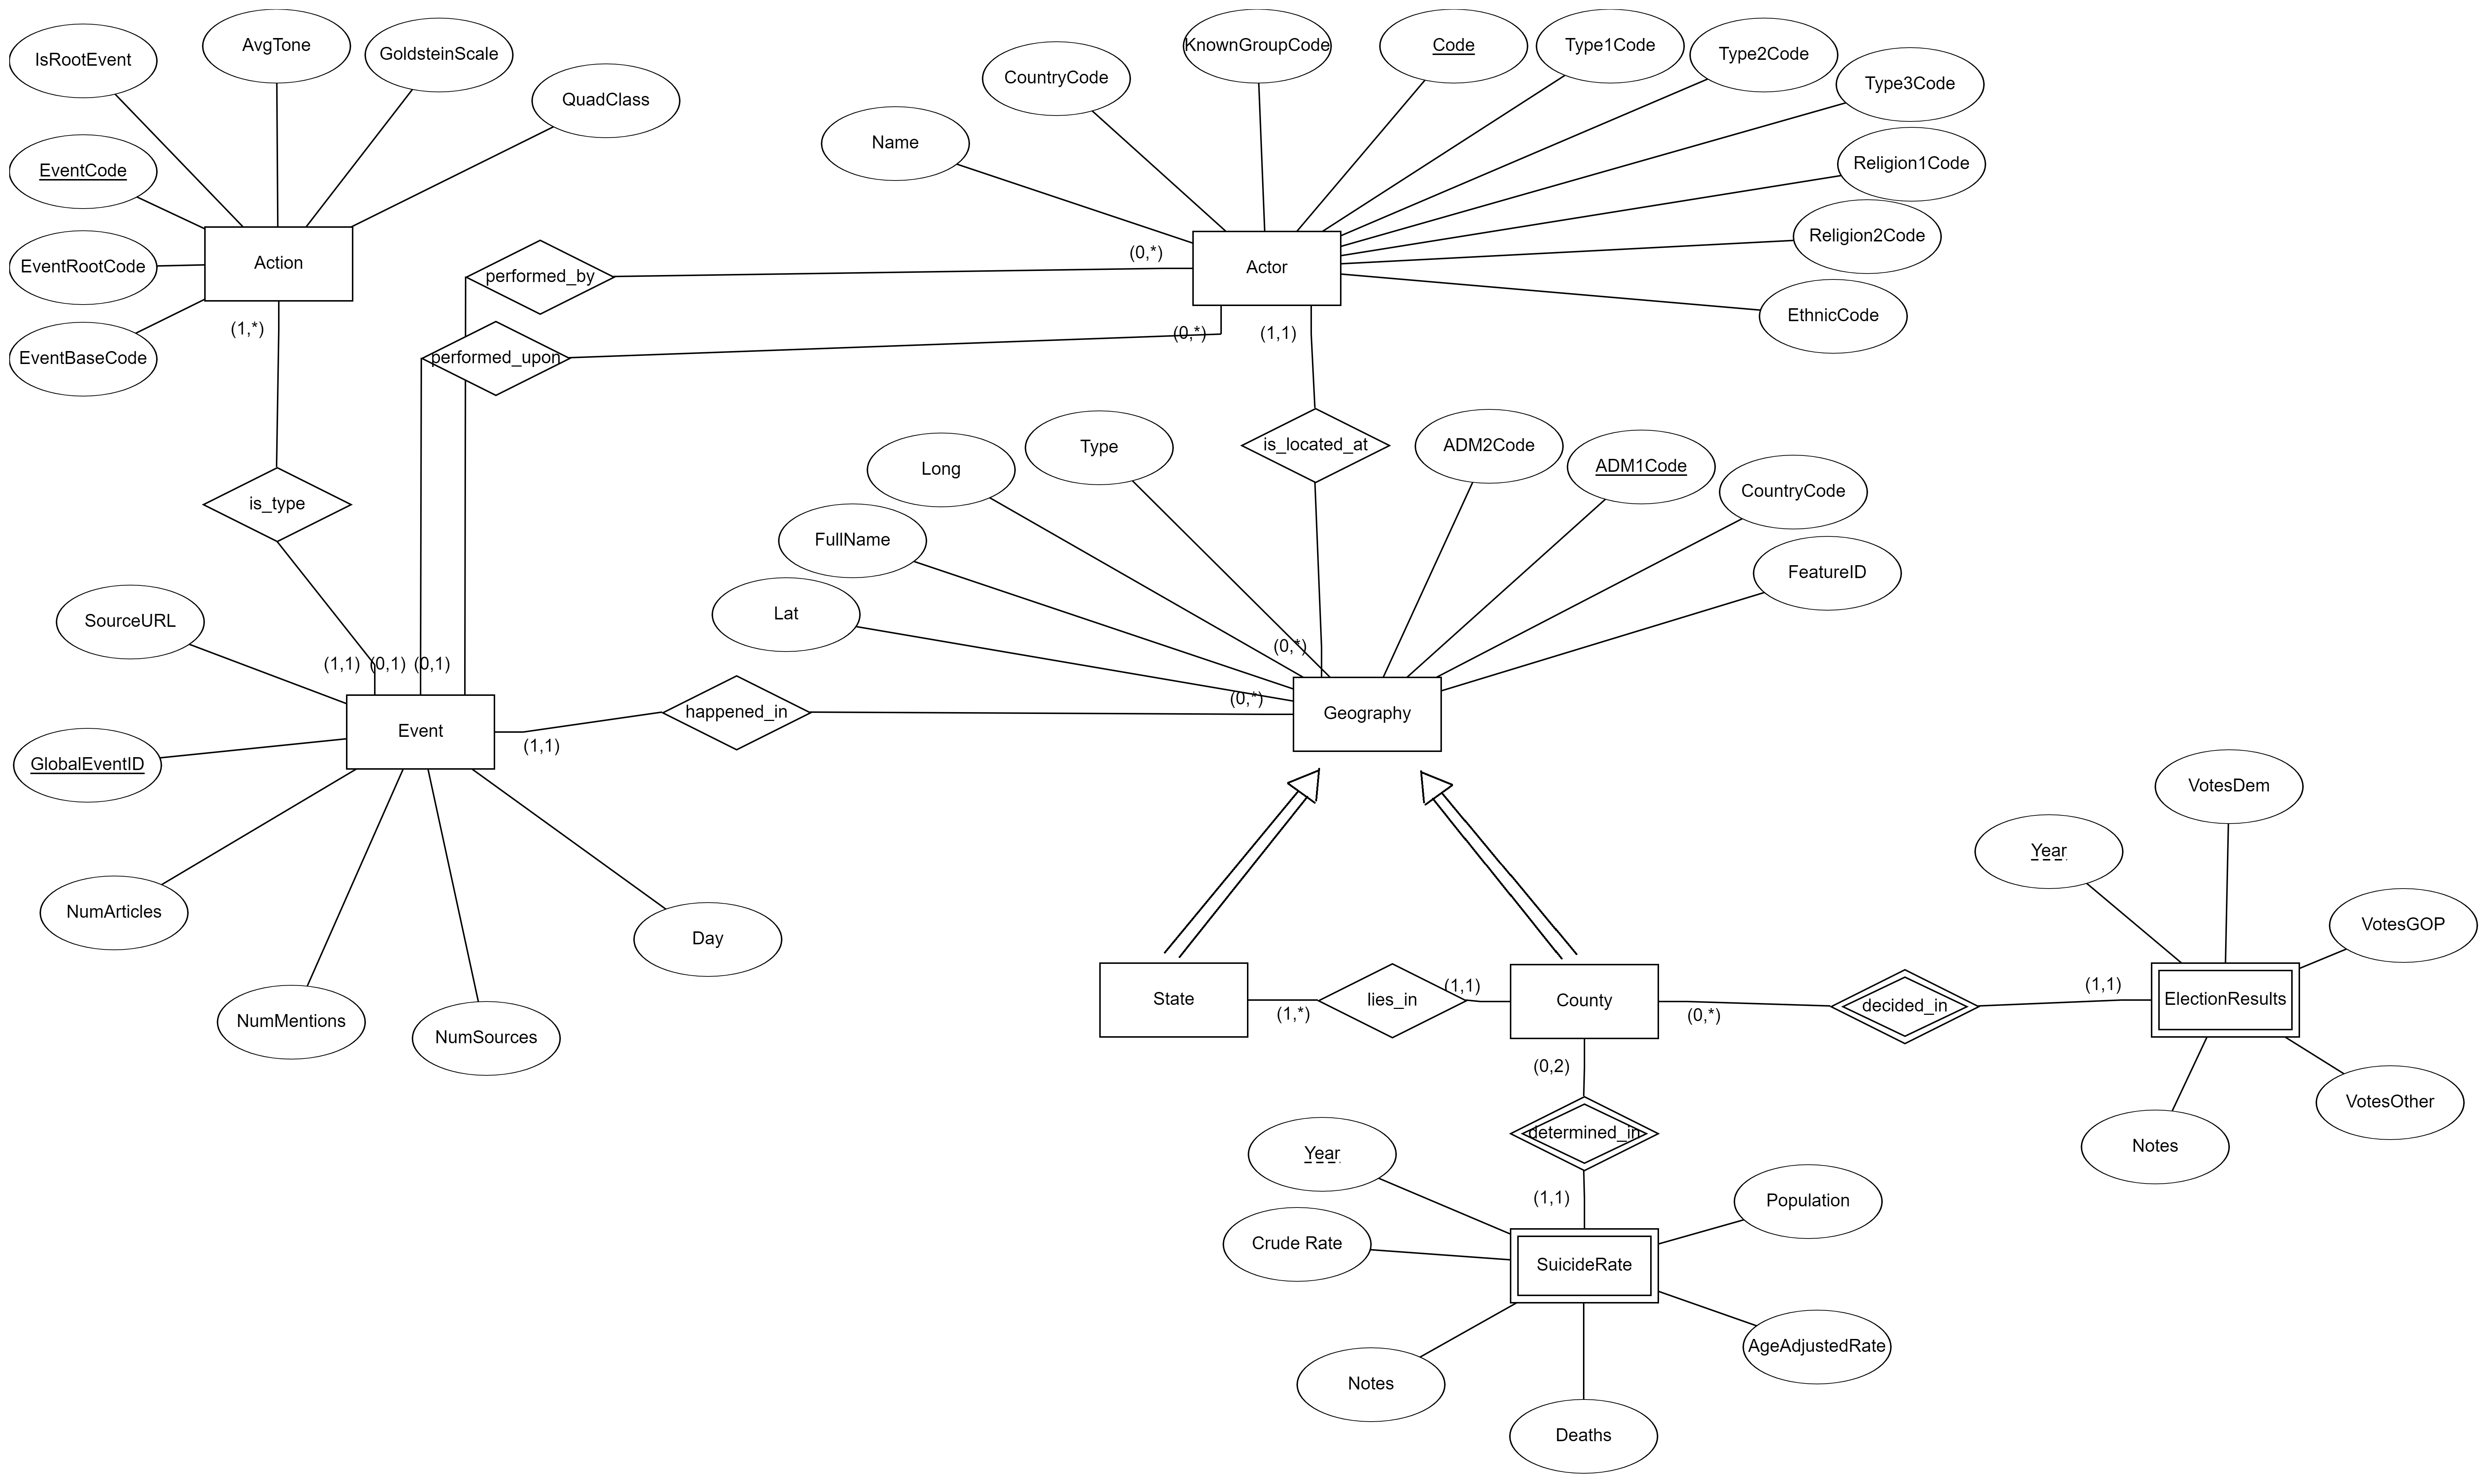
\includegraphics[scale = 0.08]{g9-all}
	\caption{Schema over the whole database}
	\label{fig:all}
\end{figure}


\textbf{Putting it all together}:
The election results and the Suicide Rate data sets have the
county attribute in common.
A county lies in a state, and both a county and a state are
spesializations of a "geography".
Some other attributes can be removed since they are redundant
(e.g. MonthYear makes the Year attribute irrelevant).
The end result can be seen on figure \ref{fig:all}.

\textbf{Technical parts}
On the inegration process, we tried using the counties' FIPS codes
present on each of the datasets to link the different entities
together.
However we quickly learned that each dataset's FIPS code
contradicts the FIPS code each other data set.

Our solution has been to identify each county (and state)
by a geoID code than can be derived from {\color{red}{todo
https://community.esri.com/thread/24614
ESRI
}}.

The only other hazard occurs when ElectionResults generates an
ID that does not match any County, in that case the corresponding
row is simply skipped and also printed to STDOUT for reference.


\section{DATA ANALYSIS}
The main and most important part.
We use sql queries to filter out the data that we need, make a bunch of plots and document everything.
We try to be as objective as possible.

%The main and most important part.
We use sql queries to filter out the data that we need, make a bunch of plots and document everything.
We try to be as objective as possible.


\section{INTERPRETATION}
Why are the results the way they are?

%Why are the results the way they are?


\section{CONCLUSION}
final words

%final words



\bibliographystyle{ieeetr}
\bibliography{references}
%\printbibliography
\end{document}
